   
\documentclass[11pt]{article}
\renewcommand{\baselinestretch}{1.05}
\usepackage{amsmath,amsthm,verbatim,amssymb,amsfonts,amscd, graphicx}
\usepackage{graphics}
\topmargin0.0cm
\headheight0.0cm
\headsep0.0cm
\oddsidemargin0.0cm
\textheight23.0cm
\textwidth16.5cm
\footskip1.0cm
\theoremstyle{plain}
\newtheorem{theorem}{Theorem}
\newtheorem{corollary}{Corollary}
\newtheorem{lemma}{Lemma}
\newtheorem{proposition}{Proposition}
\newtheorem*{surfacecor}{Corollary 1}
\newtheorem{conjecture}{Conjecture} 
\newtheorem{question}{Question} 
\theoremstyle{definition}
\newtheorem{definition}{Definition}
\usepackage{subcaption} 

\usepackage{graphicx}


 \begin{document}
 


\title{Homework 2 Machine Learning}
\date{}
\author{Marco Treglia}
\maketitle

\section{Linear Regression}
Simple linear regression is a statistical method that allows us to summarize and study relationships between two continuous (quantitative) variables:

One variable, denoted x, is regarded as the predictor, explanatory, or independent variable.
The other variable, denoted y, is regarded as the response, outcome, or dependent variable.


\section{Mathematical step}
\subsection{Linear regression}
Since we are interested in summarizing the trend between two quantitative variables, the natural question arises — "what is the best fitting line?"
In order to examine which of the two lines is a better fit, we first need to introduce some common notation:


$y_{i}$  denotes the observed response for experimental unit $i$

$x_{i}$  denotes the predictor value for experimental unit $i$

$y\hat{}_{i}$  is the predicted response (or fitted value) for experimental unit i


Then, the equation for fitting line is:

$$y\hat{}_{i} =w_{0}+w_{1} x_{i}  $$


For computing $w_{0} $ and  $w_{1} $  we need first calculate the correlation $r_{xy}$, the standar deviation $\sigma$ and the mean $\mu$ of  $x_{i} $ and $y_{i}$ :


$$ r_{xy\; }=\frac{\sum_{i=1}^{n}{\left( x_{i}\; -\; \overline{x} \right)\left( y_{i}\; -\; \overline{y} \right)}}{\sqrt{\sum_{i=1}^{n}{\left( x_{i}\; -\; \overline{x} \right)^{2}\sum_{i=1}^{n}{\left( y_{i}\; -\; \overline{y} \right)^{2}}}}}$$

$$\sigma \; \; =\; \sqrt{\frac{1}{N}\sum_{i=1}^{n}{\left( x_{i}\; -\; \mu  \right)^{2}}}$$

Then $w_{1} $ and  $w_{0} $ are : 

$$ w_{1}\; =\; r_{xy}\; \frac{\sigma _{x}}{\sigma _{y}}\;  $$

$$ w_{0}\; =\; \mu _{y}\; -\; w_{1\; }\mu _{x}\; $$

Another way for computing $w_{0} $ and  $w_{1} $  is with the linear squares minimization , wich is computationally less expensive: 

$$\arg \; \min _{w}\; \sum_{i}^{}{\left( y_{i}\; -\; wx_{i} \right)^{2}} $$



We  find  $w_{1} $ and  $w_{0} $ are : 

$$w_{1}\; \; =\; \frac{\sum_{i}^{}{x_{i}y_{i}}}{\sum_{i}^{}{x_{i}^{2}}}$$

$$w_{0}\; \; =\; \frac{\sum_{i}^{}{y_{i}}-\; w_{1}x_{i}}{n}$$

\subsection{Polynomial regression}
Polynomial regression is used to fit nonlinear (e.g. curvilinear) data into a least squares linear regression model. It is a form of linear regression that allows one to predict a single y variable by decomposing the x variable into a nth order polynomial.

$$y\; =\; w_{o}\; +\; w_{1}x\; +\; .\; .\; .\; +\; w_{k}x^{n}$$ 

In order to evaluate how good is the predicted response we can measure the MSE (Mean Square Error). The result can be interpreted as the mesure of the accuracy of our model, the smaller it's the better way  the model behaving.
$$M\mbox{SE}\; =\; \frac{1}{n}\sum_{i=1}^{n}{\left( y_{i}\; -\; y\hat{}_{i} \right)^{2}}$$

\section{Linear and Polynomial  Regression Visualizzation}

\subsection{Data}

\begin{center}
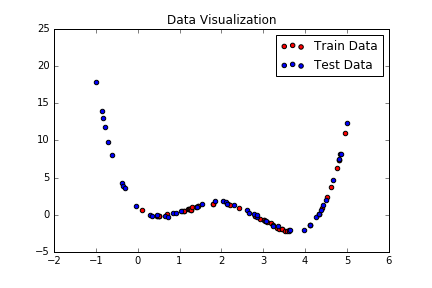
\includegraphics[scale=0.4]{00}
\end{center}


\subsection{Linear Regression}

\begin{center}
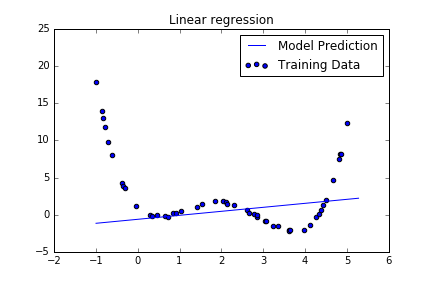
\includegraphics[scale=0.4]{0}


MSE : 38.194
\end{center}


\subsection{Polynomial Regression}

\begin{center}
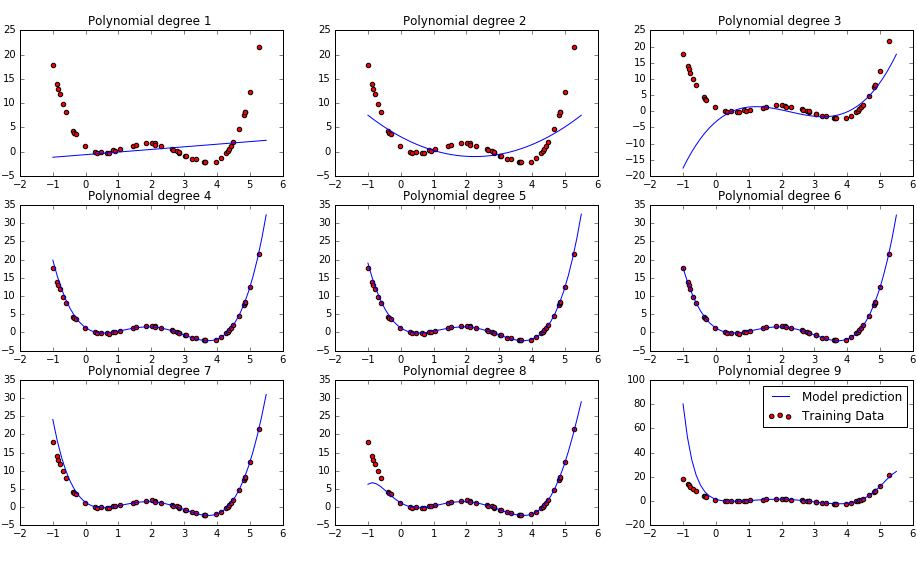
\includegraphics[scale=0.5]{1}
\end{center}


\begin{center}
 \begin{tabular}{||c c||} 
 \hline
 Polynomial degree &  MSE\\ [0.3ex] 
 \hline\hline
 1 & 38.1943  \\ 
 \hline
 2 & 14.0058 \\
 \hline
 3 & 95.6221 \\
 \hline
 4 & 0.31226 \\ 
 \hline
 5 & 0.13625 \\ 
 \hline
 6 &  0.02608 \\ [2ex]
 \hline
 7 & 1.98759 \\
 \hline
 8 & 5.44563  \\
 \hline
 9 & 157.243\\ 
 \hline
\end{tabular}
\end{center}

\begin{center}
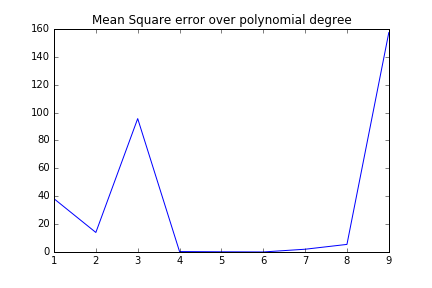
\includegraphics[scale=0.5]{3}
\end{center}


\end{document}